\newpage
\pdfbookmark[1]{\infoname}{info} % Adding the info page among the PDF bookmarks


% English information
\begin{info}
\begin{abstract}
\textit{Andmejälgija} is a protocol developed by Information System Authority (RIA), the purpose of which is to provide a uniform interface for querying Estonian residents' data access logs. There is also an \textit{Andmejälgija} web-view accessible from the state-portal eesti.ee. 

The purpose of this thesis is to create a mobile application that would notify it's users of updates in the access logs, letting them know that their data in some state database has been accessed. Implementation choices of different aspects of the solution are also going to be covered together with advantages and disadvantages of each. Additionaly, the overview of the existing state databases will be provided, including whether they provide access logs or not.
\end{abstract}

% Visual abstract is not required for all curricula
%\begin{visualAbstract}
%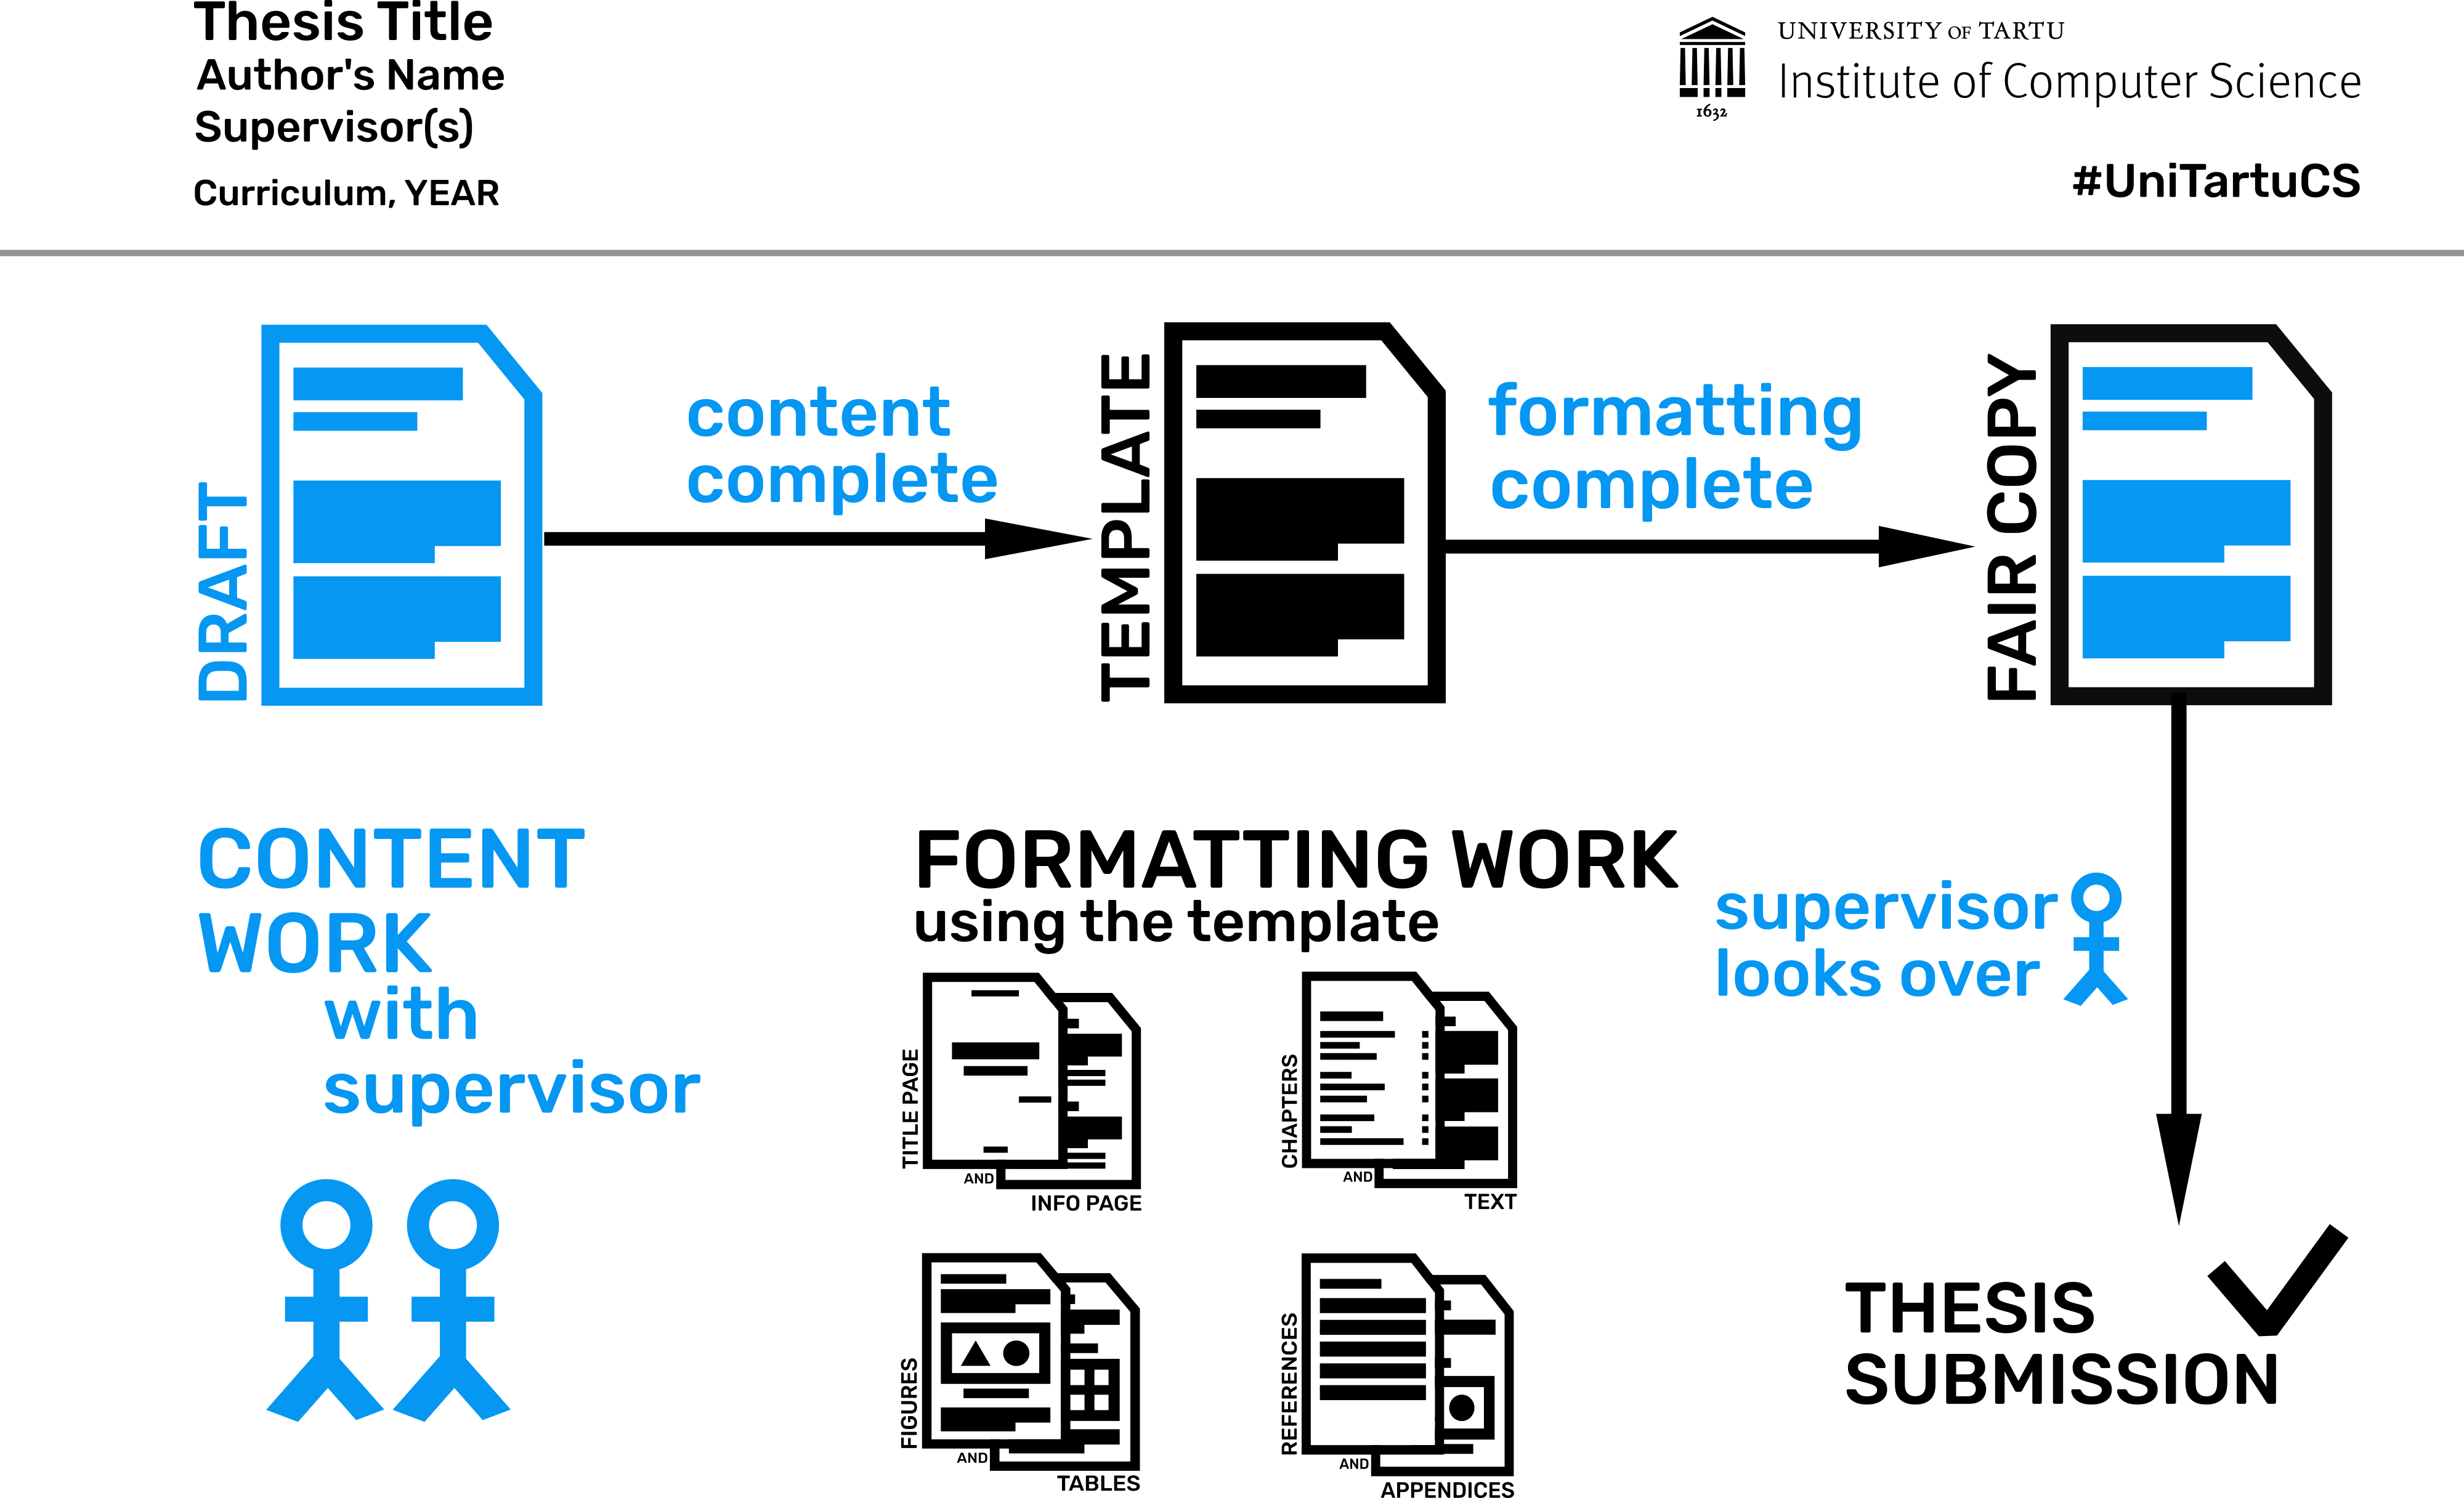
\includegraphics[width=\textwidth]{figures/Figure0-VisualAbstract.png}
%\end{visualAbstract}

% \keywords{}

\cercs{T180 Telecommunication engineering }
% Codes can be found at: https://www.etis.ee/Portal/Classifiers/Index/26
% Example: P170 Computer science, numerical analysis, systems, control
% Example: P175 Informatics, systems theory
\end{info}



% Estonian information
\begin{otherInfo}{estonian}{Andmejälgija teavitaja}
\begin{abstract}
Käesoleva lõputöö eesmärk on luua rakendus, mis teavitaks kasutajaid juurdepääsulogide uuendustest, andes neile teada, et nende andmeid mõnes riigi andmebaasis on kasutatud. Rakendusel on olnud erinevad rakendusvariandid, mida käsitletakse ka koos igaühe eeliste ja puudustega. Lisaks antakse ülevaade olemasolevatest riiklikest andmebaasidest, sealhulgas sellest, kas nad pakuvad juurdepääsulogisid või mitte.
\end{abstract}

% Visual abstract is not required for all curricula
%\begin{visualAbstract}
%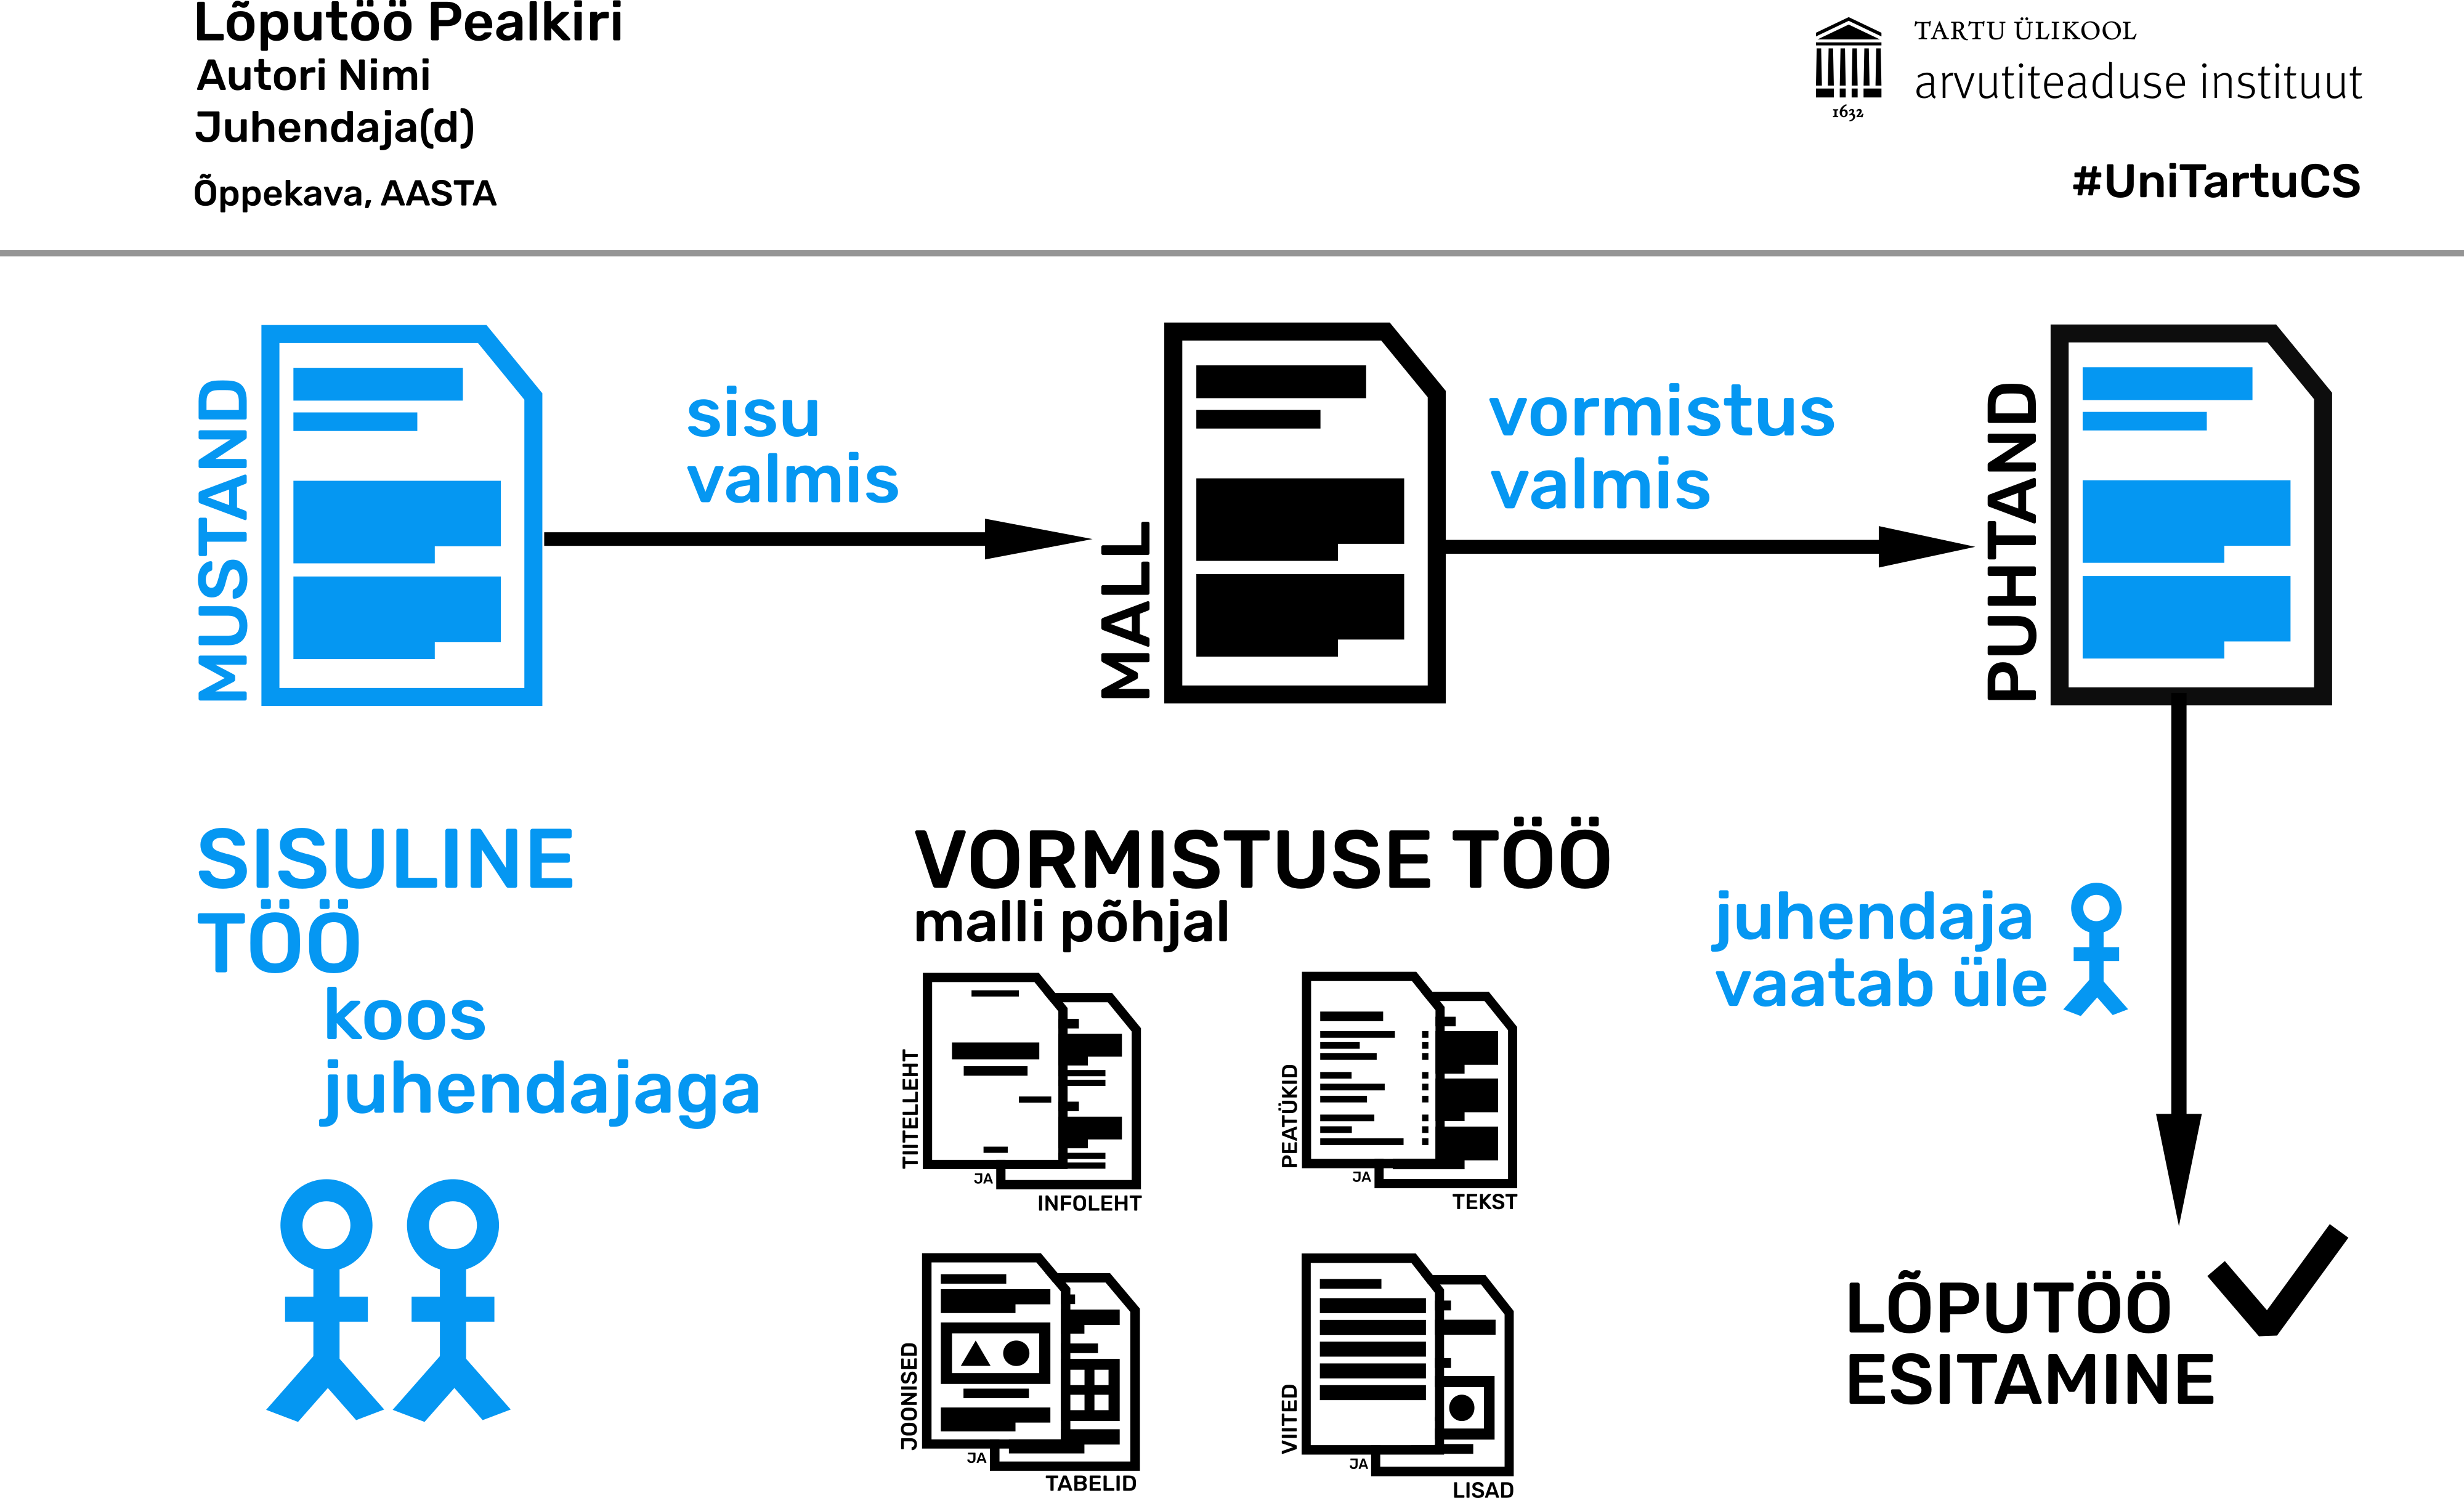
\includegraphics[width=\textwidth]{figures/Figure0-VisualAbstract-est.png}
%\end{visualAbstract}

% \keywords{}

\cercs{T180 Telekommunikatsioonitehnoloogia}
\end{otherInfo}

